\documentclass[]{report}[12 pt]
\usepackage{geometry}
\usepackage{amsmath}
\usepackage{graphicx}
\usepackage{hyperref}
\geometry{margin= 1.5 cm}
\begin{document}
	\begin{titlepage}
	\begin{center}
		\vspace*{1cm}
		
		\Huge
		\textbf{Laboratory Report}
		
		\vspace{0.5cm}
		\LARGE
		X Ray Diffraction\\
		\vspace{0.5cm}
		\textbf{Guide: Prof. Sangita Bose}
		
		\vspace{1.5cm}
		
		\textbf{A R Bathri Narayanan}\\
		Roll no: P0211501\\
		UM DAE Centre for Excellence in Basic Sciences
		
		\vspace{3 cm}
		
		Report presented for the\\
		Advanced Physics Laboratory Course (PL 701)
		
		\vspace{0.8cm}
		
		
\includegraphics[width=0.4\textwidth]{cebs.jpg}
		
		\Large
		School of Physical Sciences\\
		UM-DAE Centre for Excellence in Basic Sciences\\
		Mumbai, MH, India\\
		\today
		
	\end{center}
\end{titlepage}
	\section*{Objectives:}
	\begin{enumerate}
	\item To study the theory of X Ray diffraction, and use it on the given crystal (Lithium Fluoride)
	\item To use different X-Rays (Copper and Molybdenum) and obtain the spectrum and hence the wavelength
	\item To use a filter (Nickel for Copper and Zirconium for Molybdenum) and find out it's effects on the spectrum
	\item To find out the structure of the given material (Copper).
	\end{enumerate}
	\section*{Apparatus required}
	X Ray diffractometer, a crystal of Li-F, Cu and Mo metal targets, Computer for analysis and measuring.
	\section*{Theory}
A strong method for figuring out a crystalline material's atomic and molecular structure is X-ray diffraction, which is employed in materials science and crystallography. X-rays experience diffraction when they come into contact with a crystalline material, producing a distinctive pattern of dispersed X-rays. Details regarding the arrangement of atoms or molecules within the crystal are contained in this pattern.\\
In most cases, X-rays produced by an X-ray tube are used for X-ray diffraction. An X-ray tube accelerates high-energy electrons before they crash with a metal target, such molybdenum or copper. These collisions cause X-rays to be released.\\
Certain wavelengths of distinctive X-rays are generated, which are dictated by the target material's electron transitions. The energy of these X-rays is appropriate for diffraction experiments.\\
We mainly use the \textbf{Bragg's law of diffraction} which states
\[2dsin\theta = n\lambda\]
Where\\
\begin{itemize}
	\item $\lambda$ is the incident wavelength
	\item n is the order of the diffraction peak
	\item $\theta$ is the angle of incidence
	\item d is the spacing between the lattice planes
	\[d=\frac{a}{\sqrt{h^2+k^2+l^2}}\]
	\begin{center}
		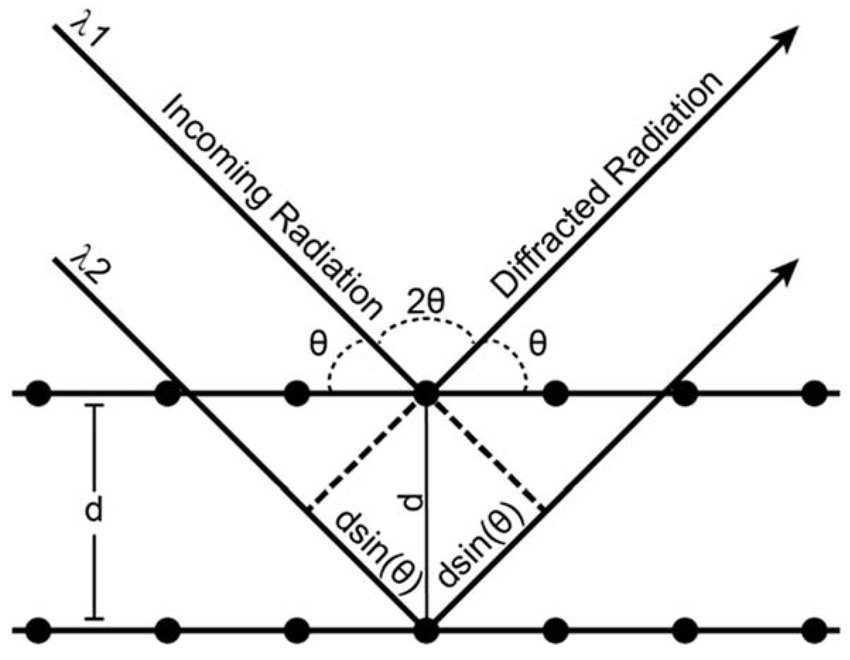
\includegraphics[width=10cm]{bragg.jpg}
	\end{center}
\end{itemize}
	\section*{Observations}
	\subsection*{Target:Copper, Crystal:LiF, Filter: None}
	We obtain a spectrum like this\\
	\begin{center}
		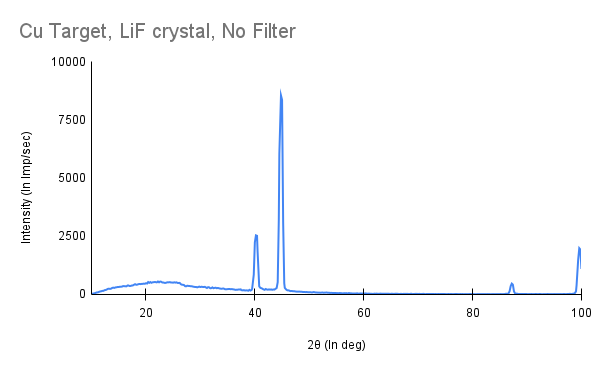
\includegraphics[width=10 cm]{Cu Target, LiF crystal, No Filter.png}\\
		\textit{Spectrum of LiF XRD with Copper Target and no filter}
	\end{center}
	We try to match it with the table given to us

		\begin{center}
		\begin{tabular}{|c|c|c|c|c|}
		\hline
		2 $\theta$ & Intensity & h & k & l \\
		\hline
		38.696 & 95 & 1 & 1 & 1 \\
		\hline
		44.996 & 100 & 2 & 0 & 0 \\
		\hline
		65.494 & 48 & 2 & 2 & 0 \\
		\hline
		78.765 & 10 & 3 & 1 & 1 \\
		\hline
		82.998 & 11 & 2 & 2 & 2 \\
		\hline
		99.628 & 3 & 4 & 0 & 0 \\
		\hline
		112.967 & 4 & 3 & 3 & 1 \\
		\hline
		117.606 & 14 & 4 & 2 & 0 \\
		\hline
		139.134 & 13 & 4 & 2 & 2 \\
		\hline
	\end{tabular}\\
	\textit{2$\theta$ vs Intensity data for Lithium Fluoride}
	\end{center}
	At the first thought, it seems like the 38.696, 44.996, to an extent 82.998 and 99.628 bands are visible. So we mark that.
	\begin{center}
		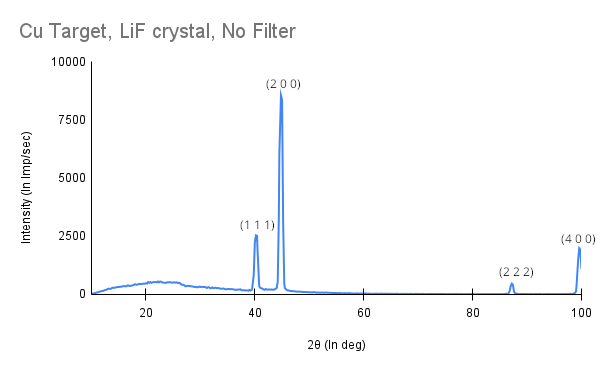
\includegraphics[width=10 cm]{a1.png}\\
		\textit{Marked spectrum of LiF XRD with Copper Target and no filter}
	\end{center}

\subsection*{Target:Copper, Crystal:LiF, Filter:Ni}
We obtain a spectrum like this\\
\begin{center}
	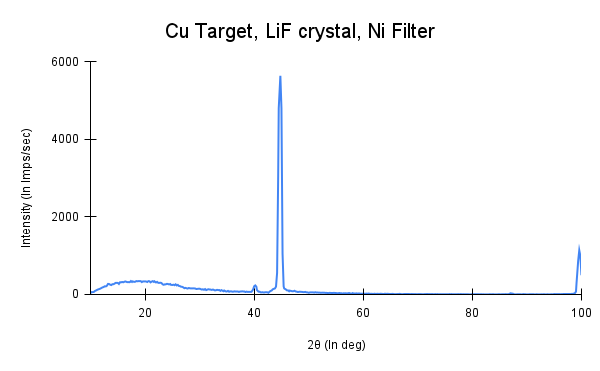
\includegraphics[width=10 cm]{Cu Target, LiF crystal, Ni Filter.png}\\
	\textit{Spectrum of LiF XRD with Copper Target and Ni filter}
\end{center}
This comes as a surprise for us as
\begin{enumerate}
	\item There is no (1 1 1) band or (2 2 2) band in the filtered one
	\item There are bands of only one kind predominant, that is the (h,0,0) type bands. We present the combined two graphs together for a better inference
		\begin{center}
		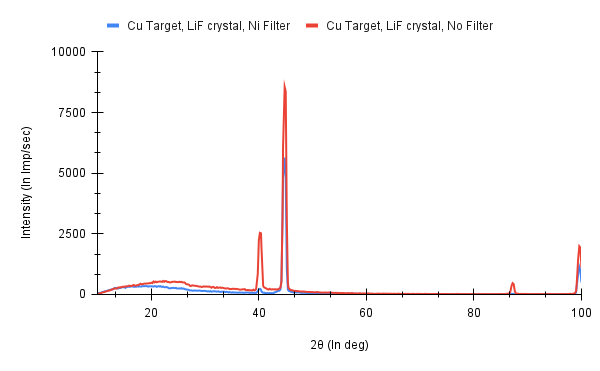
\includegraphics[width=10 cm]{comb1.png}\\
		\textit{Combined spectrum of LiF XRD and Copper Target, with and without filter}
	\end{center}
\end{enumerate}

\subsection*{Inferences}
\begin{itemize}
	\item The presence of just (h,0,0) bands should imply the crystal lattice is oriented in a single direction, hence it is a mono-crystalline solid.
	\item We can find out the wavelength of the X-Ray with this spectrum.
	We know\\
	\begin{equation*}
		2dsin\theta=n\lambda
	\end{equation*}
	We have 
	\[d=\frac{a}{\sqrt{h^2+k^2+l^2}}\]
	We have a to be 402 pm or 4.02 {\AA}  which is the lattice constant of LiF.
	Calculating the $\lambda$ of the X-Ray, we get
	\begin{align*}
		\lambda &= \frac{2\times4.02\times10^{-10}}{\sqrt{2^2+0^2+0^2}} sin(44.8/2)\\
		\lambda &= 1.531 {\AA}
	\end{align*}
	The uncertainty stems up from the least count of the machine (0.2 degrees). Accounting that\\
	\textbf{$\lambda$ = 1.531 $\pm$ 0.007 \AA}
		\item So the line which we incorrectly marked as (1 1 1) was actually the $K_{\beta}$ line, the major one being the $K_{\alpha}$ line. Doing the similar calculations for the $K_{\beta}$  line, we get
			\begin{align*}
			\lambda &= \frac{2\times4.02\times10^{-10}}{\sqrt{2^2+0^2+0^2}} sin(40.2/2)\\
			\lambda &= 1.381 {\AA}
		\end{align*}
	With uncertainty, \textbf{$\lambda$ = 1.381 $\pm$ 0.007 \AA}
	Now finally marking both the spectrum with the correct markings
	\begin{center}
	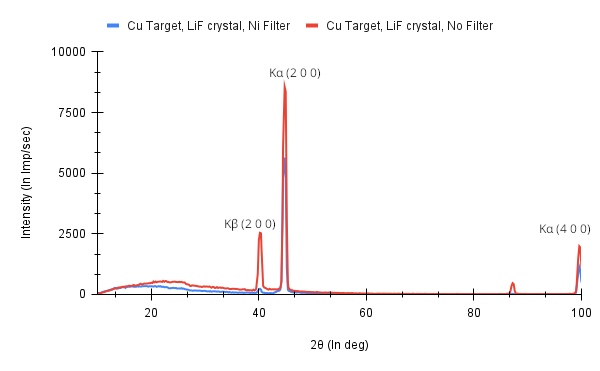
\includegraphics[width=10cm]{a2.png}
	\end{center}
\item The role of the filter is that it shunts away the $K_{\beta}$ line, hence we get only the $K_{\alpha} $ spectrum.
	\end{itemize}

\subsection*{Target:Molybdenum, Crystal:LiF, Filter: None}
We obtain a spectrum like this\\
\begin{center}
	\includegraphics[width=10 cm]{Mo Target, LiF crystal, No Filter.png}\\
	\textit{Spectrum of LiF XRD with Molybdenum Target and no filter}
\end{center}
We try to match it with the table given to us

\begin{center}
	\begin{tabular}{|c|c|c|c|c|}
		\hline
		2 $\theta$ & Intensity & h & k & l \\
		\hline
		17.548 & 95 & 1 & 1 & 1 \\
		\hline
		20.295 & 100 & 2 & 0 & 0 \\
		\hline
		28.843 & 48 & 2 & 2 & 0 \\
		\hline
		33.971 & 10 & 3 & 1 & 1 \\
		\hline
		35.525 & 11 & 2 & 2 & 2 \\
		\hline
		41.251 & 3 & 4 & 0 & 0 \\
		\hline
		45.146 & 4 & 3 & 3 & 1 \\
		\hline
		46.387 & 14 & 4 & 2 & 0 \\
		\hline
		51.119 & 13 & 4 & 2 & 2 \\
		\hline
	\end{tabular}\\
	\textit{2$\theta$ vs Intensity data for Lithium Fluoride}
\end{center}
Similar to case with Copper, it seems like there is a (1 1 1) band. But we shall not mark it this time, being a bit more cautious.

\subsection*{Target:Molybdenum, Crystal:LiF, Filter:Ni}
We obtain a spectrum like this\\
\begin{center}
	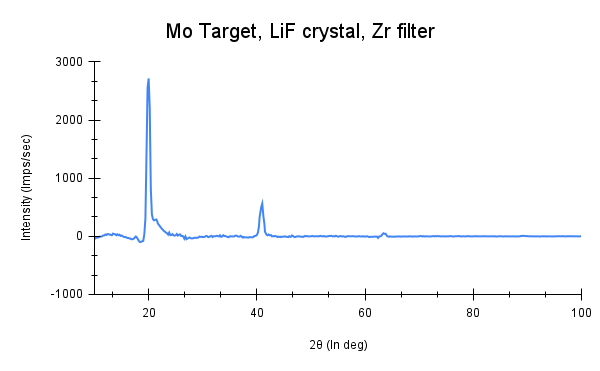
\includegraphics[width=10 cm]{a3.png}\\
	\textit{Spectrum of LiF XRD with Copper Target and Ni filter}
\end{center}
This was expected this time, to nail the points once more
\begin{enumerate}
	\item There is no (1 1 1) band or (2 2 2) band in the filtered one
	\item There are bands of only one kind predominant, that is the (h,0,0) type bands. We present the combined two graphs together for a better inference
	\begin{center}
		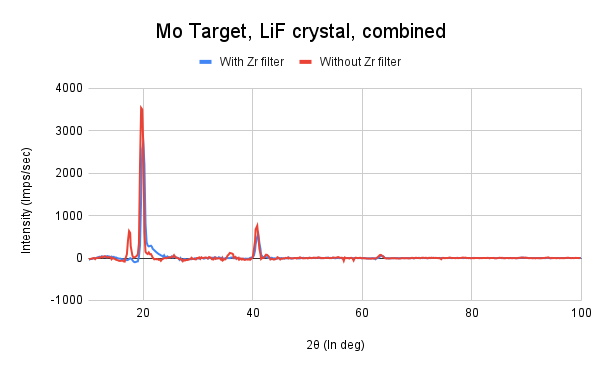
\includegraphics[width=10 cm]{comb2.png}\\
		\textit{Combined spectrum of LiF XRD and Copper Target, with and without filter}
	\end{center}
\end{enumerate}

We do the same analysis once more
\subsection*{Inferences}
\begin{itemize}
	\item The presence of just (h,0,0) bands should imply the crystal lattice is oriented in a single direction, hence it is a mono-crystalline solid.
	\item We can find out the wavelength of the X-Ray with this spectrum.
	We know\\
	\begin{equation*}
		2dsin\theta=n\lambda
	\end{equation*}
	We have 
	\[d=\frac{a}{\sqrt{h^2+k^2+l^2}}\]
	We have a to be 402 pm or 4.02 {\AA}  which is the lattice constant of LiF.
	Calculating the $\lambda$ of the X-Ray, we get
	\begin{align*}
		\lambda &= \frac{2\times4.02\times10^{-10}}{\sqrt{2^2+0^2+0^2}} sin(20/2)\\
		\lambda &= 0.698 {\AA}
	\end{align*}
	The uncertainty stems up from the least count of the machine (0.2 degrees). Accounting that\\
	\textbf{$\lambda$ = 0.698 $\pm$ 0.007 \AA}
	\item So the line which we incorrectly marked as (1 1 1) was actually the $K_{\beta}$ line, the major one being the $K_{\alpha}$ line. Doing the similar calculations for the $K_{\beta}$  line, we get
	\begin{align*}
		\lambda &= \frac{2\times4.02\times10^{-10}}{\sqrt{2^2+0^2+0^2}} sin(17.6/2)\\
		\lambda &= 0.615 {\AA}
	\end{align*}
	With uncertainty, \textbf{$\lambda$ = 0.615 $\pm$ 0.007 \AA}
	Now finally marking both the spectrum with the correct markings
	\begin{center}
		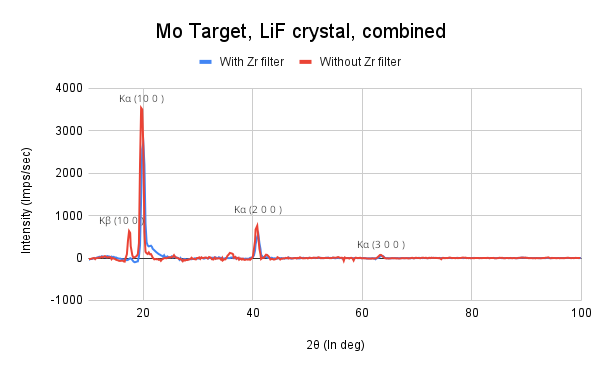
\includegraphics[width=10cm]{combm2.png}
	\end{center}
	\item The role of the filter is that it shunts away the $K_{\beta}$ line, hence we get only the $K_{\alpha} $ spectrum.
\end{itemize}

\subsection*{Target:Copper, Crystal:Cu, Filter: Ni}
Now we know the wavelength of the X-Ray (1.531 $\pm$ 0.007 {\AA}) when a copper target is used, we now try to find the structure of Copper using this. We also use this as an opportunity to switch the plotting software to GNUplot.
\begin{center}
	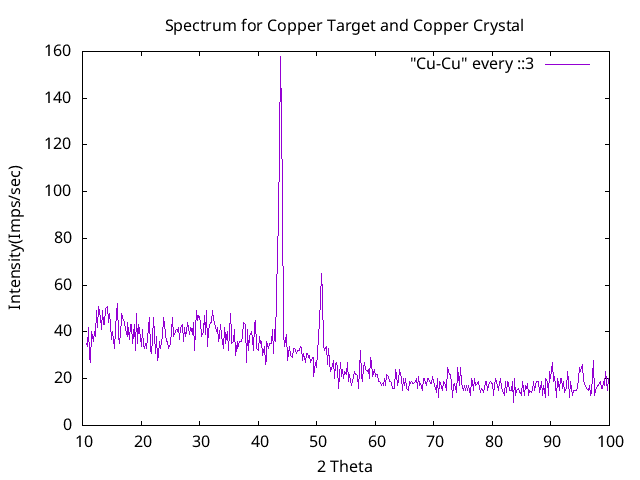
\includegraphics[width=10 cm]{cucu.png}
\end{center}
We refer the table for Copper
\begin{center}
	\begin{tabular}{|c|c|c|c|c|}
		\hline
		2$\theta$ & Intensity & h & k & l \\
		\hline
		43.297 & 100 & 1 & 1 & 1 \\
		\hline
		50.433 & 46 & 2 & 0 & 0 \\
		\hline
		74.130 & 20 & 2 & 2 & 0 \\
		\hline
		89.931 & 17 & 3 & 1 & 1 \\
		\hline
		95.139 & 5 & 2 & 2 & 2 \\
		\hline
		116.919 & 3 & 4 & 0 & 0 \\
		\hline
		136.507 & 9 & 3 & 3 & 1 \\
		\hline
		144.714 & 8 & 4 & 2 & 0 \\
		\hline
	\end{tabular}
\end{center}
Now we try labelling the peaks, there is a peak at 43.8, 50.8. The other peaks are shadowed by noise.
\begin{center}
	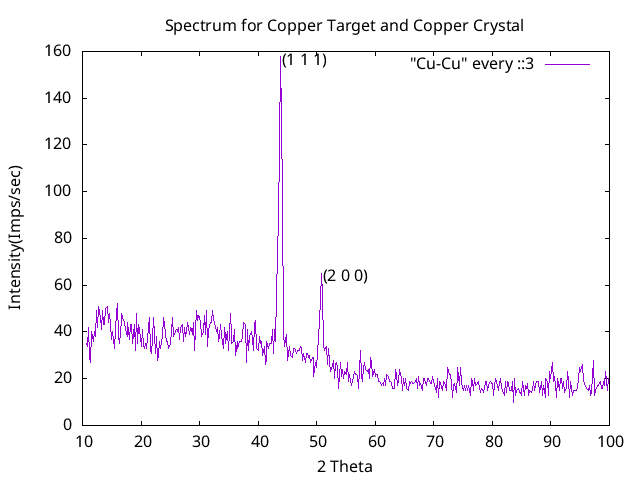
\includegraphics[width=10 cm]{cucu1.png}
\end{center}
Since there are two different planes present, this is a polycrystalline sample. Now we try to find the lattice parameter.
	\begin{equation*}
	2dsin\theta=n\lambda
\end{equation*}
We have 
\[d=\frac{a}{\sqrt{h^2+k^2+l^2}}\]
So we can rearrange as
\[d=\frac{n\lambda}{2sin\theta}\]
\[a=\frac{\lambda}{2sin\theta}\times\sqrt{h^2+k^2+l^2}\]
Plugging in $\lambda=1.531{\AA}, \theta=21.9^{\circ}, \sqrt{h^2+k^2+l^2} =\sqrt{3}$.
\[a=3.554{\AA}\]
Plugging in $\lambda=1.531{\AA}, \theta=25.4^{\circ}, \sqrt{h^2+k^2+l^2} =\sqrt{4}$
\[a=3.569{\AA}\]
Error obtained = $\pm$ 0.003{\AA}
\subsection*{Target:Copper, Crystal:Si, Filter: Ni}
Next we try to analyse the Silicon crystal given to us.
\begin{center}
	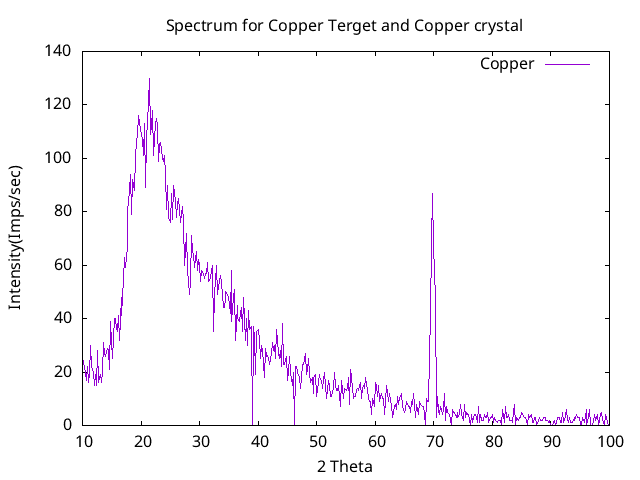
\includegraphics[width=10cm]{cusi.png}
\end{center}
At the first sight, the right side of spectrum is noisy, suggesting contamination. Which was suspected as the Silicon crystal looked dirty. Looking at the database, we have peaks visible at 27.8 and 69.8. All the other potential peaks are subsumed by noise and impurities.\\
\begin{center}
	\begin{tabular}{|c|c|c|c|c|}
		\hline
		2$\theta$ & Intensity & h & k & l \\
		\hline
		28.443 & 100 & 1 & 1 & 1 \\
		\hline
		47.304 & 55 & 2 & 2 & 0 \\
		\hline
		56.122 & 30 & 3 & 1 & 0 \\
		\hline
		69.132 & 6 & 4 & 0 & 0 \\
		\hline
		76.379 & 11 & 3 & 3 & 1 \\
		\hline
		88.029 & 12 & 4 & 2 & 2 \\
		\hline
		 94.957 & 6 & 5 & 1 & 1 \\
		\hline
	\end{tabular}\\
	Si database
	The higher values of $2\theta$ are excluded due to instrument measuring only till $2\theta=100$
\end{center}
\begin{center}
	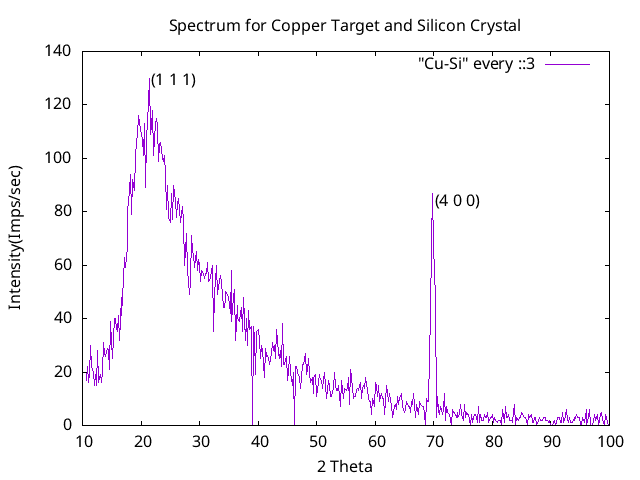
\includegraphics[width=10 cm]{cusi1.png}
\end{center}
Since there are two different planes present, this is a polycrystalline solid.Now we try to find the lattice parameter.
\begin{equation*}
	2dsin\theta=n\lambda
\end{equation*}
We have 
\[d=\frac{a}{\sqrt{h^2+k^2+l^2}}\]
So we can rearrange as
\[d=\frac{n\lambda}{2sin\theta}\]
\[a=\frac{\lambda}{2sin\theta}\times\sqrt{h^2+k^2+l^2}\]
 Plugging in $\lambda=1.531{\AA}, \theta=13.9, \sqrt{h^2+k^2+l^2} =\sqrt{3}$.
 \[a=5.519{\AA}\]
 Plugging in $\lambda=1.531{\AA}, \theta=34.9, \sqrt{h^2+k^2+l^2} =\sqrt{16}$
 \[a=5.35{\AA}\]
 Error obtained = $\pm$ 0.003{\AA}
  \section*{Result}
 \begin{enumerate}
 	\item The X-Ray wavelength of Copper target is 
 	\begin{itemize}
 		\item 	$K_{\alpha}$\textbf{= 1.531 $\pm$ 0.007 \AA}
 		\item 	$K_{\beta}$\textbf{= 1.381 $\pm$ 0.007 \AA}
 	\end{itemize}
\item The X-Ray wavelength of Molybdenum target is 
 	\begin{itemize}
 		\item 	$K_{\alpha}$\textbf{= 0.698 $\pm$ 0.007 \AA}
 		\item 	$K_{\beta}$\textbf{= 0.615 $\pm$ 0.007 \AA}
 	\end{itemize}
 	\item We analysed a Copper crystal (Supposedly FCC)
\begin{enumerate}
\item Lattice parameter for (h h h) plane = \textbf{= 3.554 $\pm$ 0.003 \AA}
\item Lattice parameter for (h 0 0) plane = \textbf{= 3.569 $\pm$ 0.003 \AA}
\end{enumerate}
 	\item We analysed an impure Silicon crystal (Supposedly Diamond)
\begin{enumerate}
	\item Lattice parameter for (h h h) plane = \textbf{= 5.519 $\pm$ 0.003 \AA}
	\item Lattice parameter for (h 0 0) plane = \textbf{= 5.351 $\pm$ 0.003 \AA}
\end{enumerate}
 \end{enumerate}
\end{document}